%% bare_conf.tex
%% V1.4b
%% 2015/08/26
%% by Michael Shell
%% See:
%% http://www.michaelshell.org/
%% for current contact information.
%%
%% This is a skeleton file demonstrating the use of IEEEtran.cls
%% (requires IEEEtran.cls version 1.8b or later) with an IEEE
%% conference paper.
%%
%% Support sites:
%% http://www.michaelshell.org/tex/ieeetran/
%% http://www.ctan.org/pkg/ieeetran
%% and
%% http://www.ieee.org/

%%*************************************************************************
%% Legal Notice:
%% This code is offered as-is without any warranty either expressed or
%% implied; without even the implied warranty of MERCHANTABILITY or
%% FITNESS FOR A PARTICULAR PURPOSE! 
%% User assumes all risk.
%% In no event shall the IEEE or any contributor to this code be liable for
%% any damages or losses, including, but not limited to, incidental,
%% consequential, or any other damages, resulting from the use or misuse
%% of any information contained here.
%%
%% All comments are the opinions of their respective authors and are not
%% necessarily endorsed by the IEEE.
%%
%% This work is distributed under the LaTeX Project Public License (LPPL)
%% ( http://www.latex-project.org/ ) version 1.3, and may be freely used,
%% distributed and modified. A copy of the LPPL, version 1.3, is included
%% in the base LaTeX documentation of all distributions of LaTeX released
%% 2003/12/01 or later.
%% Retain all contribution notices and credits.
%% ** Modified files should be clearly indicated as such, including  **
%% ** renaming them and changing author support contact information. **
%%*************************************************************************


% *** Authors should verify (and, if needed, correct) their LaTeX system  ***
% *** with the testflow diagnostic prior to trusting their LaTeX framework ***
% *** with production work. The IEEE's font choices and paper sizes can   ***
% *** trigger bugs that do not appear when using other class files.       ***                          ***
% The testflow support page is at:
% http://www.michaelshell.org/tex/testflow/


\label{beginning of document}
\documentclass[10pt,conference]{IEEEtran}
% Some Computer Society conferences also require the compsoc mode option,
% but others use the standard conference format.
%
% If IEEEtran.cls has not been installed into the LaTeX system files,
% manually specify the path to it like:
% \documentclass[conference]{../sty/IEEEtran}

\usepackage{makecell}
\usepackage[noadjust]{cite}
\usepackage{graphicx}
	\graphicspath{{images/}} 
\renewcommand\IEEEkeywordsname{Keywords}
\usepackage{hyperref}
	\hypersetup{colorlinks=true,allcolors=blue}
\usepackage{hypcap}
\usepackage{caption}
\usepackage{subcaption}
\usepackage{listings}
\lstset{
 		basicstyle=\ttfamily\scriptsize,
 		%frame=single,
 		breaklines=true,
 		numbers=left,
 		xleftmargin=2.5em,
 		framexleftmargin=0em,
 		emph={
       	class, extends, operation, abstract,
       	context, constraint, check,
       	for, if, return, true, and, ref,
       	message, in, package, val, attr, 
       	@link, @node, @compartment,
       	@namespace, @diagram
   	},
   	emphstyle=\textbf
}
\lstdefinestyle{interfaces}{
 		float=t
}
\lstdefinestyle{xmi}{
    basicstyle=\ttfamily\scriptsize,
    emph={
        X, A, B, C, Class, Package    
    }
}
\lstdefinestyle{eol}{
    basicstyle=\ttfamily\scriptsize,
    emph={
        var, new, for, in, create, set, of, with, 
        unset, to, add, remove, delete, register, move,
        from, position, from, move-within, session, \.
    }
}

\lstdefinestyle{java}{
    basicstyle=\ttfamily\scriptsize,
    emph={
        case, $unset$,
        instanceof, else, if, void,
        new, UnsetEAttributeEvent,
        UnsetEReferenceEvent,
        @override, public, class, extends
    }
}

% correct bad hyphenation here
\hyphenation{op-tical net-works semi-conduc-tor}
\newcommand{\dk}[1]{\textbf{[Dimitris: #1]}}

\begin{document}
%
% paper title
% Titles are generally capitalized except for words such as a, an, and, as,
% at, but, by, for, in, nor, of, on, or, the, to and up, which are usually
% not capitalized unless they are the first or last word of the title.
% Linebreaks \\ can be used within to get better formatting as desired.
% Do not put math or special symbols in the title.
\title{Towards Hybrid Model Persistence}


% author names and affiliations
% use a multiple column layout for up to three different
% affiliations\ref{abstract}
\author{\IEEEauthorblockN{Alfa Yohannis\IEEEauthorrefmark{1}, Horacio Hoyos Rodriguez\IEEEauthorrefmark{2}, Fiona Polack\IEEEauthorrefmark{3}, Dimitris Kolovos\IEEEauthorrefmark{4}}
\IEEEauthorblockA{
    \IEEEauthorrefmark{1}\IEEEauthorrefmark{2}\IEEEauthorrefmark{4}Department of Computer Science, University of York, United Kingdom \\
    \IEEEauthorrefmark{3}School of Computing and Maths, Keele University, United Kingdom \\
Email: \IEEEauthorrefmark{1}ary506@york.ac.uk, \IEEEauthorrefmark{2}horacio\_hoyos\_rodriguez@ieee.org, \\
\IEEEauthorrefmark{3}f.a.c.polack@keele.ac.uk, \IEEEauthorrefmark{4}dimitris.kolovos@york.ac.uk}}

% conference papers do not typically use \thanks and this command
% is locked out in conference mode. If really needed, such as for
% the acknowledgment of grants, issue a \IEEEoverridecommandlockouts
% after \documentclass

% for over three affiliations, or if they all won't fit within the width
% of the page, use this alternative format:
% 
%\author{\IEEEauthorblockN{Michael Shell\IEEEauthorrefmark{1},
%Homer Simpson\IEEEauthorrefmark{2},
%James Kirk\IEEEauthorrefmark{3}, 
%Montgomery Scott\IEEEauthorrefmark{3} and
%Eldon Tyrell\IEEEauthorrefmark{4}}
%\IEEEauthorblockA{\IEEEauthorrefmark{1}School of Electrical and Computer Engineering\\
%Georgia Institute of Technology,
%Atlanta, Georgia 30332--0250\\ Email: see http://www.michaelshell.org/contact.html}
%\IEEEauthorblockA{\IEEEauthorrefmark{2}Twentieth Century Fox, Springfield, USA\\
%Email: homer@thesimpsons.com}
%\IEEEauthorblockA{\IEEEauthorrefmark{3}Starfleet Academy, San Francisco, California 96678-2391\\
%Telephone: (800) 555--1212, Fax: (888) 555--1212}
%\IEEEauthorblockA{\IEEEauthorrefmark{4}Tyrell Inc., 123 Replicant Street, Los Angeles, California 90210--4321}}




% use for special paper notices
%\IEEEspecialpapernotice{(Invited Paper)}




% make the title area
\maketitle

% As a general rule, do not put math, special symbols or citations
% in the abstract
\begin{abstract}
\label{abstract}
In contrast to state-based model persistence approaches (e.g. XMI, NeoEMF) that store snapshots of the state of a model conforming to a 3-level metamodelling architecture such as EMF, change-based approaches persist its complete -- and ever-growing -- editing history instead. Change-based persistence has the potential to support faster and more accurate model comparison, merging, as well as a range of analytics activities. On the other hand, reconstructing the state of a model by replaying its editing history every time the model needs to be queried or modified can get increasingly expensive as the model grows in size. In this work, we integrate change-based and state-based persistence mechanisms in a hybrid model persistence approach that delivers the best of both worlds. In this  paper, we present the design of our hybrid model persistence approach and report on its impact on time and memory footprint for model loading and saving, storage space usage, and model differencing.
\end{abstract}
%
% no keywords
\begin{IEEEkeywords} 
model persistence, hybrid model persistence, change-based model persistence, state-based model persistence, model comparison
\end{IEEEkeywords}

% For peer review papers, you can put extra information on the cover
% page as needed:
% \ifCLASSOPTIONpeerreview
% \begin{center} \bfseries EDICS Category: 3-BBND \end{center}
% \fi
%
% For peerreview papers, this IEEEtran command inserts a page break and
% creates the second title. It will be ignored for other modes.
\IEEEpeerreviewmaketitle

\vspace{-5pt}
\section{Introduction}
\label{sec:introduction}
Change-based persistence (CBP) of models conforming to metamodelling architectures such as MOF/EMF \cite{DBLP:conf/models/YohannisKP17} comes with notable advantages over state-based persistence (SBP): it provides support for fast comparison and differencing of versions of the same model \cite{DBLP:conf/sde/LippeO92,DBLP:conf/caise/IgnatN05,DBLP:conf/edoc/KoegelHLHD10,koegel2010emfstore}  -- which can also substantially speed up incremental model management activities, and enables novel model analytics activities (e.g. pattern detection in the editing history to understand how modellers use modelling languages and tools) \cite{DBLP:journals/entcs/RobbesL07}. However, CBP comes at the cost of ever-growing model files \cite{DBLP:conf/edoc/KoegelHLHD10,DBLP:journals/entcs/RobbesL07} since all changes (even deleting model elements) are recorded in an ever-longer editing log, which naturally leads to longer loading times \cite{mens2002state}. In this work we address the latter challenge by introducing the concept of hybrid persistence of models. In hybrid persistence (HP) the change-based representation is augmented with a fully-derived (what do you mean by fully derived?), state-based representation of the latest state of the model which is used to speed up model loading and querying.
 
The rest of the paper is structured as follows. Section \ref{sec:change_and_state_based_model_persistence} introduces the concept of change-based model persistence and recent work on state-based model persistence. Section \ref{sec:hybrid_model_persistence} presents our approach to hybrid model persistence. Section \ref{sec:evaluation} presents experimental results and evaluation. Section \ref{sec:related_work} provides an overview of related work, and Section \ref{sec:conlcusions_and_future_work} concludes with a discussion on directions for future work.

\section{Change and State-based Model Persistence}
\label{sec:change_and_state_based_model_persistence}
To explain the differences, benefits and drawbacks of CBP and SBP, consider a modelling activity on a UML model as presented Fig. \ref{fig:illustration_cbp}. The sub-figures $a$ to $h$ depict the evolution of a UML model at different time stamps. It can be seen that classes are created ad added/removed from \texttt{Package X}. Adding a class involves creating the new class and then settings its name. 

In SBP only the final state of the model is persisted. Thus, to represent the final state of the UML model, only the information about \texttt{Package X} and \texttt{Class C} needs to be persisted, as presented in Lst. \ref{lst:xmimodel2} (XMI format). In CBP all the changes in the model are persisted. Thus, a list of all the changes (events) in the model are needed to represent the final state of the model, as presented in Lst. \ref{lst:cbpmodel}\footnote{We use a natural language pseudo-code of the CBP format introduced in \cite{DBLP:conf/models/YohannisKP17,yohannis2018towards}}.  A session depicts a set of changes that where done between save events, i.e. a session contains all the changes that happened since the last time (the last session) the model was persisted. Lines 2-3 represent the initial state (Fig. \ref{fig:illustration_1}), followed by lines 4-5 (Fig. \ref{fig:illustration_2}), 6-7 (Fig. \ref{fig:illustration_3}), 8 (Fig. \ref{fig:illustration_4}), 9 (Fig. \ref{fig:illustration_5}), 11 (Fig. \ref{fig:illustration_6}),12 (Fig. \ref{fig:illustration_7}), and 13 (Fig. \ref{fig:illustration_1}). 


%we use two successive versions of a UML2 \cite{eclipse2017uml2} model persisted in the state-based XMI format: the first one is the initial version (List. \ref{lst:xmimodel1}), and the second one is the update version (Fig. \ref{lst:xmimodel2}). To construct the first version of the model, a package is created and its name is set to ``X''. Two classes also created and their names are set to ``A'' and ``B''. Both classes are then added to the package. The model is then saved and produces a state-based model as presented in List. \ref{lst:xmimodel1}. In the second session, the model is modified by renaming the class `B'' to ``C'' and removing the class ``A'' from its package and deleting it entirely from the model. After that, the model is saved again to produce the second version of the model as presented in List. \ref{lst:xmimodel2}. The visual illustration of these series of modification is depicted in Fig. \ref{fig:illustration_cbp}.

%\begin{lstlisting}[style=xmi,caption={The initial version of the UML2 example model in (simplified) XMI.},label=lst:xmimodel1]
%<uml:Package xmi:id="1" name="X">
%   <packagedElement xsi:type="uml:Class" xmi:id="2" name="A"/>
 %  <packagedElement xsi:type="uml:Class" xmi:id="3" name="B"/>
%</uml:Package>
%\end{lstlisting}

\begin{lstlisting}[style=xmi,caption={The second version of the UML2 example model.},label=lst:xmimodel2]
<uml:Package xmi:id="1" name="X">
    <packagedElement xsi:type="uml:Class" xmi:id="3" name="C"/>
</uml:Package>
\end{lstlisting}

\begin{figure}[ht]
    %row 1
    \begin{subfigure}[t]{0.49\linewidth}
        \centering
        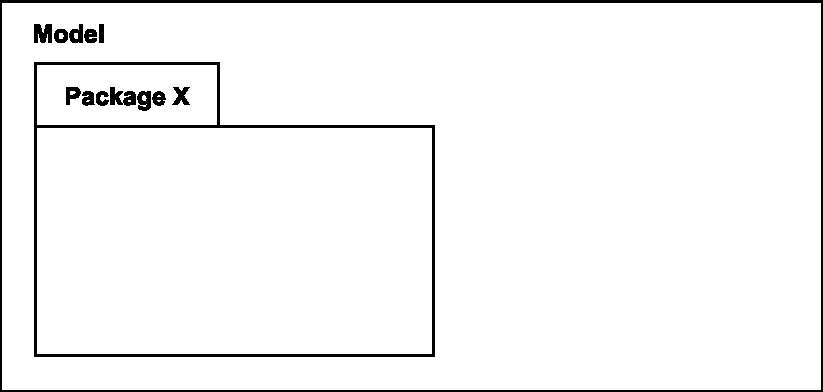
\includegraphics[width=\linewidth]{images/illustration_1}
        \caption{Initial state}
        \label{fig:illustration_1}
    \end{subfigure}
    \hfill
    \begin{subfigure}[t]{0.49\linewidth}
        \centering
        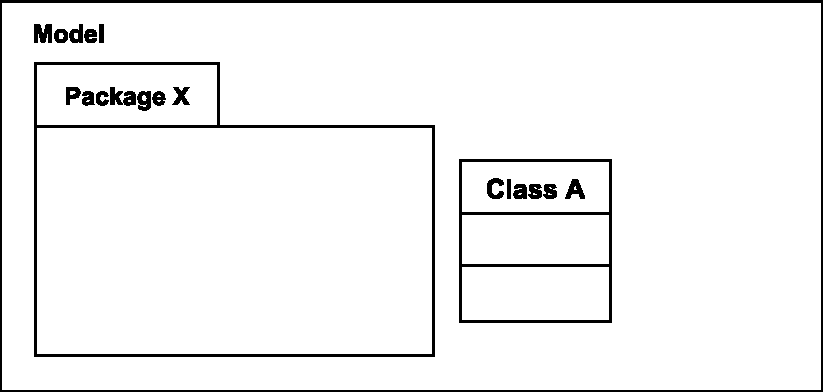
\includegraphics[width=\linewidth]{images/illustration_2}
        \caption{Time stamp 1}
        \label{fig:illustration_2}
    \end{subfigure}
    %row 2
    \begin{subfigure}[t]{0.49\linewidth}
        \centering
        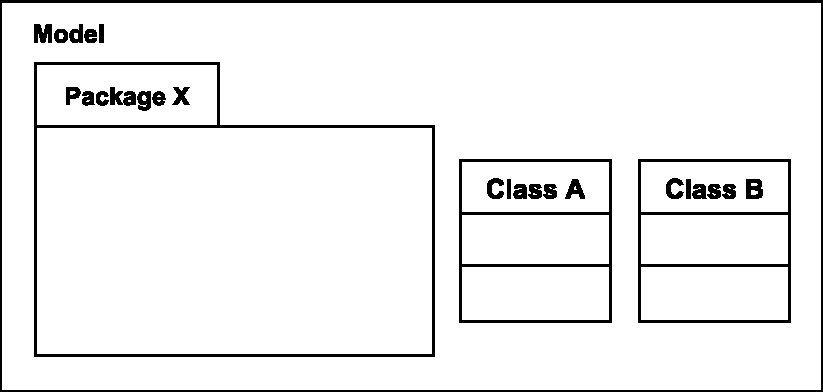
\includegraphics[width=\linewidth]{images/illustration_3}
        \caption{Time stamp 2}
        \label{fig:illustration_3}
    \end{subfigure}
    \hfill
    \begin{subfigure}[t]{0.49\linewidth}
        \centering
        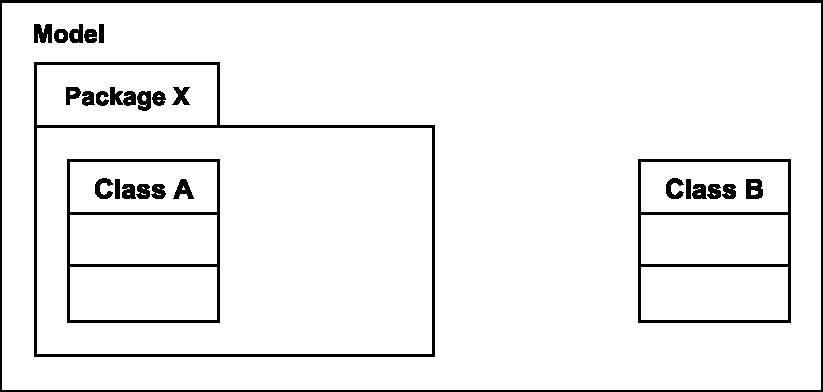
\includegraphics[width=\linewidth]{images/illustration_4}
        \caption{Time stamp 3}
        \label{fig:illustration_4}
    \end{subfigure}
    %row 3
    \begin{subfigure}[t]{0.49\linewidth}
        \centering
        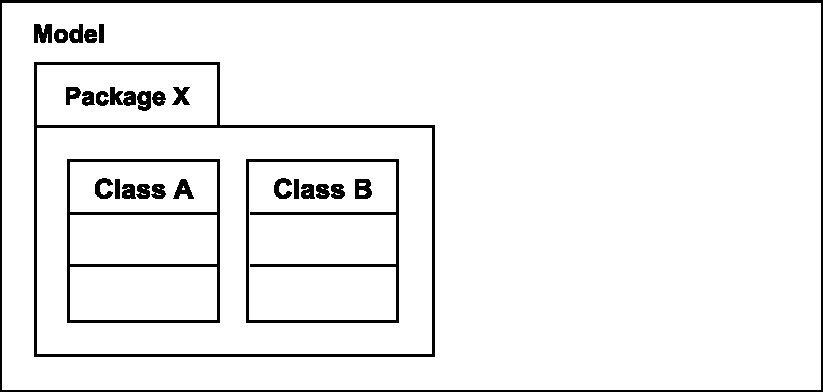
\includegraphics[width=\linewidth]{images/illustration_5}
        \caption{Time stamp 4}
        \label{fig:illustration_5}
    \end{subfigure}
    \hfill
    \begin{subfigure}[t]{0.49\linewidth}
        \centering
        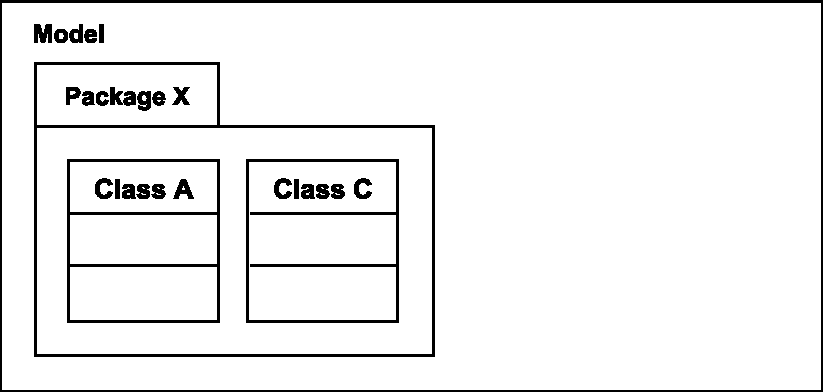
\includegraphics[width=\linewidth]{images/illustration_6}
        \caption{Time stamp 5}
        \label{fig:illustration_6}
    \end{subfigure}
    %row 4
    \begin{subfigure}[t]{0.49\linewidth}
        \centering
        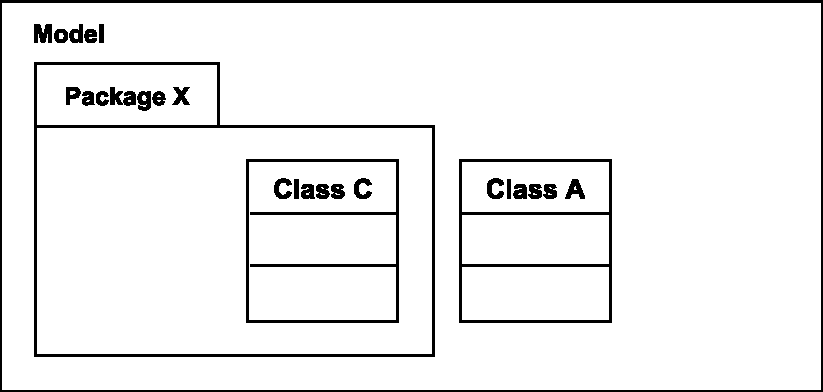
\includegraphics[width=\linewidth]{images/illustration_7}
        \caption{Time stamp 6}
        \label{fig:illustration_7}
    \end{subfigure}
    \hfill
    \begin{subfigure}[t]{0.49\linewidth}
        \centering
        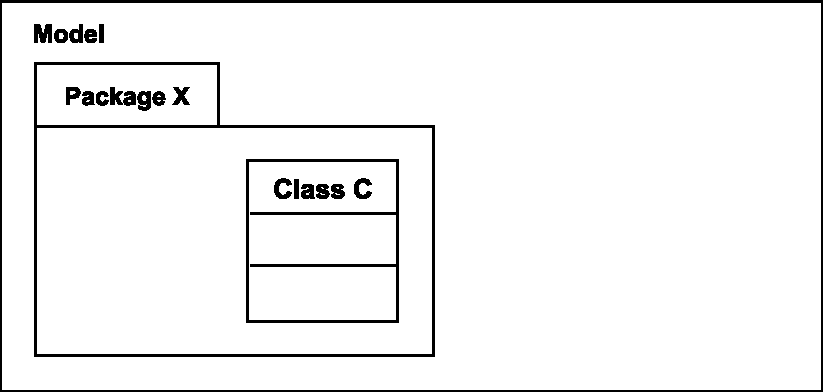
\includegraphics[width=\linewidth]{images/illustration_8}
        \caption{Time stamp 7}
        \label{fig:illustration_8}
    \end{subfigure}
    
    \caption{The states of the example model after certain changes and their corresponding lines in List. \ref{lst:cbpmodel}.}
    \label{fig:illustration_cbp}
\end{figure}

%In change-based model persistence, instead of saving the state of the model, all the changes made to it are saved instead. Change events are collected in memory during model editing and are appended into a change-based log file when the model is saved. The changes made to the example model in both sessions can be seen in a text-based (for demonstration purposes), change-based format presented in List. \ref{lst:cbpmodel}. To load a model saved in a change-based representation, its persisted change events have to be replayed -- reenacting the construction of the model from the beginning.

\begin{lstlisting}[style=eol,caption={The text change-based persistence of producing state-based model in List. \ref{lst:xmimodel2}. Its visual illustration is in Fig. \ref{fig:illustration_cbp}.},label=lst:cbpmodel]
session 1
create p1 of Package
set p1.name to "X"  
create c1 of Class
set c1.name to "A"
create c2 of Class
set c2.name to "B"
add c1 to p1.packagedElement   
add c2 to p1.packagedElement
session 2
set c2.name to "C"
remove c1 from p1.children   
delete c1
\end{lstlisting}

To load a SBP model, only the elements in the final state must be instantiated. To load a CBP model, all the events that lead to the final state must be replayed. Loading times of a SBP model are proportional to the size of the model. On the other hand, loading times of a CBP model are proportional to the number of events. As a result, loading times of CBP models will always increase over time and are considerably longer than for SBP\,\cite{yohannis2018towards,mens2002state}. 

To store a SBP model, all the elements that exist in the final state must be persisted. To save a CBP only the changes in the last session must be persisted. Storing times of SBP models are proportional to the size of the model. Storing times of CBP models are proportional to the number of events in a session. As a result, storing times of CBP models can be considerably faster than for SBP models\,\cite{yohannis2018towards}. Storing of CBP models also requires more space as events just keep adding up. 

Comparing and finding the differences between two versions of a state-based model is an expensive ($O(N^2)$ in the general case) operation and beyond change visualisation and comprehension \cite{Kolovos:2009:DMM:1564596.1564641}, this also has a substantial impact to downstream activities such as incremental model transformation \cite{DBLP:conf/ecmdafa/OgunyomiRK15} and validation \cite{Bergmann:2011:IEM:2190078.2190132}.

By contrast, in change-based persistence, changes are first-class entities in the persisted model file and as such, model comparison and differencing is relatively inexpensive (more on this in Sec. \ref{sec:evaluation}). The main downsides of change-based persistence are ever-growing model file sizes \cite{DBLP:journals/entcs/RobbesL07,DBLP:conf/edoc/KoegelHLHD10} and ever-increasing loading times \cite{mens2002state}. Even thought an attempt has been made to reduce the loading time \cite{yohannis2018towards} by detecting, memoising and subsequently ignoring change events that have no impact to the final state of the model (i.e. that have been superseded by other events), loading time can only be reduced up to around 50\%, and is still substantially longer than that of state-based approaches. 

Table \ref{table:persistence_comparsion} summarises the benefits (+) and drawbacks (-) of change and state-based model persistence.

% On the other hand, state-based model persistence is growing on its capabilities to process large-scale models by harnessing the power of big data backend. Morsa \cite{DBLP:conf/models/Espinazo-PaganCM11} and NeoEMF \cite{daniel2016neoemf} has been able to load and query models with more than a million elements since they are able to handle model's elements partially without having to load all the elements into memory when using the standard XMI persistence. However, using these backends hindered the models to be versioned on common version control systems (e.g. Git, SVN), which is crucial for collaborative development.

\begin{table} [ht]
    \centering
    \caption{Comparison of model persistence approaches.}
    \label{table:persistence_comparsion}
    \begin{tabular}{ c c c c }
        \hline 
        \textbf{Dimensions} & \textbf{Change-based} & \textbf{State-based} \\
        \hline 
        Load Time & $-$ & $+$ \\
        Save Time & $+$ & $-$ \\
        Comparison Time & $+$ & $-$ \\
        Storage Space & $-$ & $+$ \\
        \hline 
    \end{tabular}
\end{table}

% A new approach is required to combine the benefits (+) of both approaches (fast loading and comparison) with acceptable trade-off. Thus, we proposed a hybrid model persistence -- an approach that uses change and state-based persistence side-by-side to persist models. One notable drawback for this persistence is it requires more storage space since models are saved into two types of persistence. 

\section{Hybrid Model Persistence}
\label{sec:hybrid_model_persistence}
To achieve the best of both worlds we introduce a hybrid model persistence approach which combines change-based and state-based model persistence, to work together side-by-side. An overview of the proposed approach is illustrated in Fig. \ref{fig:hybrid_persistence}.

\begin{figure}[ht]
    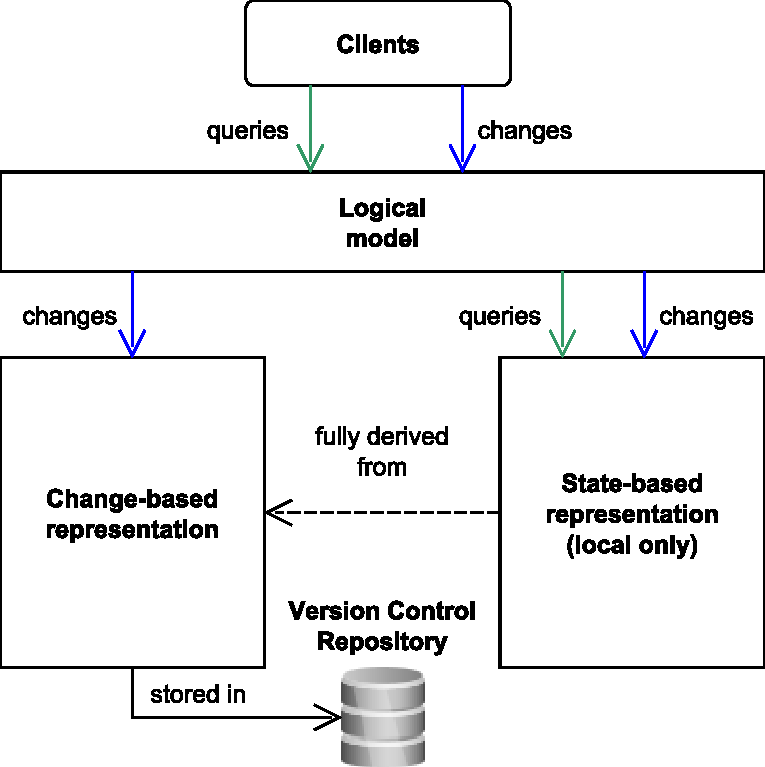
\includegraphics[width=\linewidth]{images/hybrid_persistence}
    \caption{The mechanism of the hybrid model persistence.}
    \label{fig:hybrid_persistence}
\end{figure}

In the proposed approach a \textit{hybrid} model is stored in two representations at the same time: a change-based (e.g. using CBP) and a state-based representation (e.g. using XMI or a database-backed approach such as NeoEMF). Of these representations, the change-based one is the source of truth and the state-based representation is fully derived from the former.

\paragraph{Loading a hybrid model}: Models are loaded into in-memory object graphs that clients (e.g. editors, transformations) can then interact with\footnote{Depending on the state persistence mechanism, the object graph may be loaded in its entirety at startup (e.g. XMI) or it can be loaded progressively and in a lazy manner (e.g. NeoEMF/CDO)}. In the proposed hybrid approach, if the state-based counterpart already exists, the in-memory object graph is populated from it; otherwise it is populated by replaying the complete editing history recorded in the change-based representation.

\paragraph{Changing a hybrid model}: When an element of a loaded model is created, modified or deleted, the change is applied to the in-memory object graph and is also recorded in an in-memory list of changes. We use the term \emph{editing session} for the period between loading a model and saving back to disk. 

\paragraph{Saving a hybrid model}: The current version of the in-memory object graph is stored in the preferred state-based representation, and the list of changes recorded in the current editing session is optionally compacted to remove superseded changes and appended to the change-based representation.

\paragraph{Versioning a hybrid model}: Since the state-based representation is fully derived from the change-based representation, if a model needs to be versioned (e.g. in a Git repository), only the change-based representation needs to be stored in the repository. The first time it is loaded after being checked out/cloned, the state-based representation will be computed and persisted locally and will be used in subsequent model loading steps.

\paragraph{Comparing hybrid models}: To compare two hybrid models, their change-based representations are used since, as discussed above, this is much more efficient than state-based comparison.

% When a model is modified by a client (e.g. editor, transformation program), the changes are recorded into both representations. The former persists all the changes to keep the model's history, while the latter is used to record the last state of the model produced by the changes. Changes persisted into the change-based representation are fully derived from the changes happened on the state-based representation. Since the change-based representation is text-based, it can be stored in a version control repository. In terms of querying (including loading), the model is directly queried from the state-based representation. Thus, replaying all the changes from its change-based representation to get the last state of the model -- which is time consuming -- can be avoided. This hybrid model persistence's mechanism is presented in Fig. \ref{fig:hybrid_persistence}.

\section{Implementation}
\label{sec:implementation}

We have implemented the proposed hybrid model persistence approach in a prototype on top of the Eclipse Modeling Framework (EMF) \cite{steinberg2008emf}. The prototype makes use of an existing implementation of change-based model persistence, the Epsilon CBP \cite{DBLP:conf/models/YohannisKP17}, augmented with two state-based persistence implementations: NeoEMF \cite{daniel2016neoemf} and XMI \cite{omg2018xmi}.

XMI has been selected as a standard state-based model persistence format (natively supported by EMF), and NeoEMF as a best-of-breed representative of database-backed state-based model persistence frameworks. The core components of the prototype are presented in a class diagram in Fig. \ref{fig:class_diagram}. 

\begin{figure}[ht]
    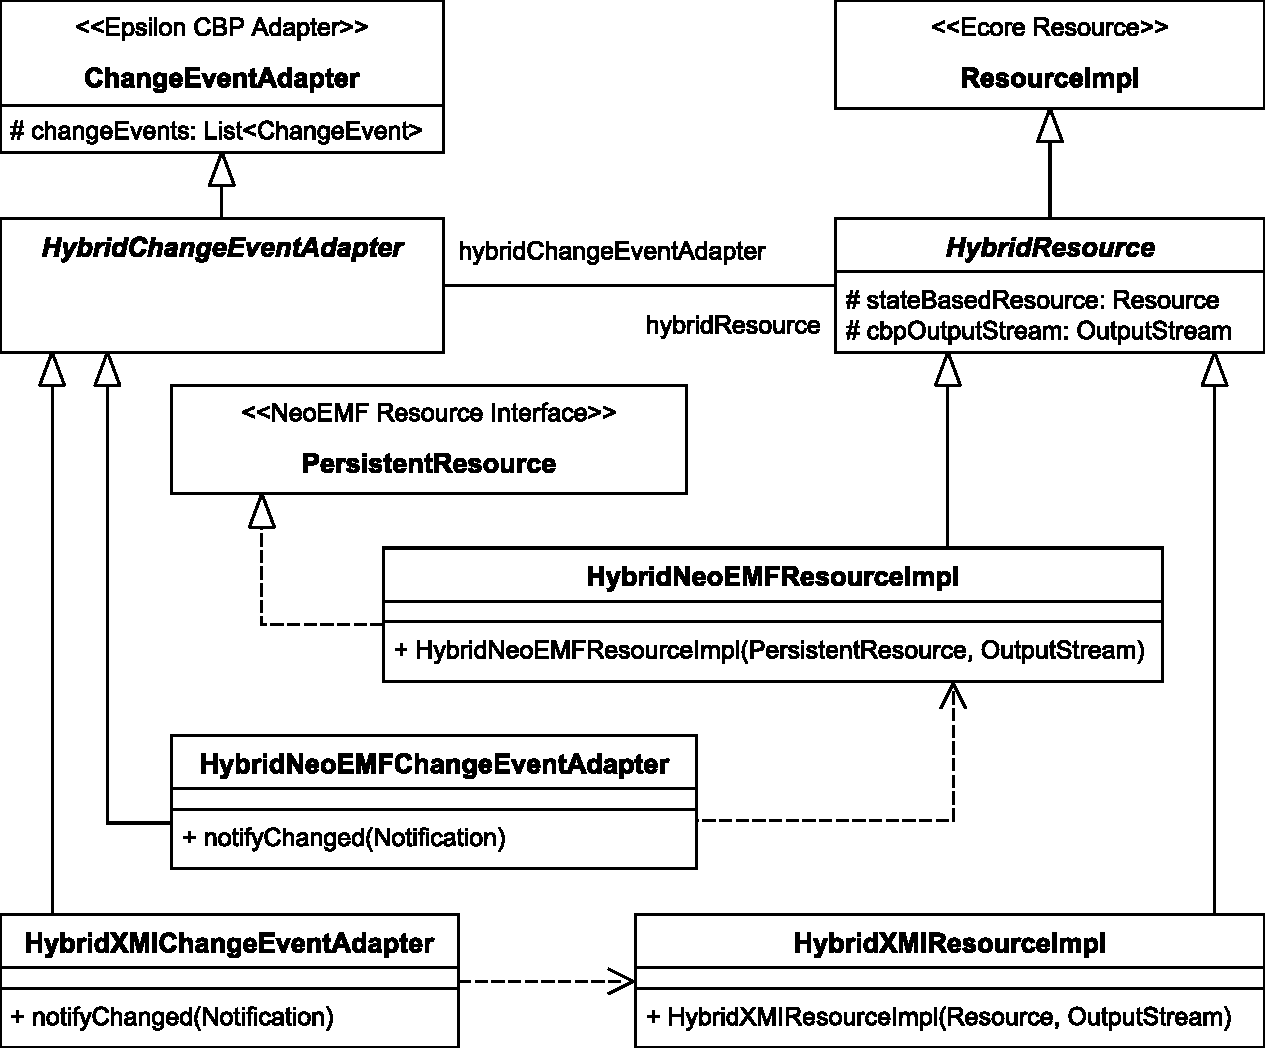
\includegraphics[width=\linewidth]{images/class_diagram}
    \caption{Core components of the hybrid model persistence implementation.}
    \label{fig:class_diagram}
\end{figure}

The Epsilon CBP provides a $ChangeEventAdapter$ class \cite{DBLP:conf/models/YohannisKP17} that is derived from the Ecore's $EContentAdapter$ adapter class \cite{eclipse2018eContentAdapter}. This class collects changes made to the in-memory object graph of an EMF model in the form of a list of events ($changeEvents$). Based on this class, we derived another adapter class, $ChangeHybridEventAdapter$, for the hybrid model persistence implementation. It is an abstract class so that it can be further derived to create different implementations of adapter classes for different types of state-based persistence. The $ChangeHybridNeoEMFEventAdapater$ is the adapter class for NeoEMF and the $ChangeHybridXMIEventAdapater$ for XMI. These classes override the $notifyChanged(Notification)$ that belongs to the $ChangeEventAdapter$ class to handle events that are specific to NeoEMF and XMI respectively.

We also created a resource class for hybrid persistence, the $HybridResource$ class (a resource class is a class dedicated to interact with a persistence, e.g. save, load, get contents), derived from the Ecore's $ResourceImpl$ \cite{eclipse2018resourceImpl}. The class is made abstract so that it can be realised in different resource implementation classes for different state-based persistence (e.g. NeoEMF and XMI). The $HybridResource$ class contains the $stateBasedResource$ field which is used to refer to a state-based persistence that is being used, and the $cbpOutputStream$ field that refers to an $OutputStream$ (e.g. file, in-memory) as the representation of the change-based persistence for saving changes. This $HybridResource$ class has an association with the $HybridChangeEventAdapater$ class so that the former can access the events collected by the latter, and the latter can also use facilities provided by the former (e.g. getting the id of an element in the resource, saving changes to a change-based model representation).

The resource implementation class for NeoEMF is the $HybridNeoEMFResourceImpl$ class, and $HybridXMIResource$$Impl$ class for XMI. Both are derived from the $HybridResource$. For $HybridNeoEMFResourceImpl$ , this class also implements the NeoEMF's $PersistenceResource$ interface \cite{atlanmod2018persistentResource} so that specific NeoEMF's methods can also be implemented on this hybrid implementation class (e.g. $close$() method to close a connection with a backend database). The complete implementation is available under \url{https://github.com/epsilonlabs/emf-cbp}.

\subsection{Known Limitations}

\dk{TODO: Discuss subset of Ecore covered, only support for single-file models, no support for detection should the state-based and change-based representations fall out of sync etc.}

\section{Evaluation}
\label{sec:evaluation}

In this section, we compare hybrid model persistence (Epsilon CBP and NeoEMF or XMI) vs. state-based persistence (NeoEMF or XMI only) on loading, saving, and storage space usage of models and argue that hybrid model persistence offers a fair trade-off for the latter. 

\subsection{Evaluation Method}
\label{sec:evaluation_method}
We developed the prototype of the proposed hybrid model persistence approach\footnote{The prototype, tests, and data used in the evaluation are available under \url{https://github.com/epsilonlabs/emf-cbp} and \url{https://goo.gl/1zUBQC}.}. The evaluation was performed on Intel\textsuperscript{\textregistered} Core\textsuperscript{TM} i7-6500U CPU@2.50GHz 2.59GHz, 12GB RAM, and the Java\textsuperscript{TM} SE Runtime Environment (build 1.8.0\textunderscore162-b12).

For the evaluation, we used models reverse-engineered from the Java source code of a real-world open-source project (Epsilon \cite{eclipse2017epsilon,eclipse2018epsilongit}). For state-based representation of the models, we used MoDisco \cite{DBLP:journals/infsof/BruneliereCDM14} to generate XMI-based UML2 \cite{eclipse2017uml2} models that reflect the classes, fields, operations of the source code of the project and then imported the generated models into NeoEMF (we also derived more UML2 models from the BPMN2 project \cite{eclipse2017bpmn2,eclipse2018bpmn2git} and MoDiscoXML \cite{eclipse2018modiscoxml} models from the United States article on Wikipedia \cite{wikipedia2018us} and used them to support the generality of our evaluation). 

While reverse-engineering a state-based representation of a model is trivial, obtaining a change-based persistence that reflects the changes it has undergone over time was not as straightforward. We performed the same procedure in \cite{yohannis2018towards} to obtain a change-based representation. The change-based representation was derived from the diffs identified from a sequence of versions of the project committed on its version control repository. From the sequential versions, different consecutive models can be generated to represent the time-ordered changes of the project. We derived the change-based representation by comparing an initially-empty running model to the generated models consecutively. All differences identified were then reconciled by performing a one-way merging to the running model. Changes to the running model in the course of the merging process were collected and then persisted into a CBP file. We used EMF Compare \cite{eclipse2017compare} to perform the comparison and merging. 

Using these models, we then evaluated the performance of our hybrid persistence prototype against XMI and NeoEMF in terms of time and memory footprint for loading, saving, and comparison/diffing of subsequent model versions using EMF Compare as the baseline for state-based comparison. %For the latter, we measured the delta of memory used before and after loading and saving completes. We also measured the impact of using the hybrid approach on the execution time of a model comparison, specifically for identifying differences between a model and its preceding version. The hybrid approach was compared to model-to-model comparison using EMF Compare on their execution time.

We repeated our experiments 22 times for each dimension measured. The results of the measurement enabled us to perform the Welch's t-test \cite{welch1947ttest} to find the significance of the comparisons for each case. We used a significance level of 5\%. % If t-test' $p$-$value$ $<$ 0.05, we rejected the null hypothesis -- the $means$ of the compared persistence types are equal ($H_0$) -- and accepted the alternative hypothesis -- the $means$ of the compared persistence types are not equal ($H_1$).  

\subsection{Loading Time and Memory Footprint}
\label{sec:model_loading_time}
In this section, we present the results of our evaluation on the time and memory footprint required for the hybrid model persistence to load a model.

\subsubsection{Epsilon Project}
\label{sec:model_loading_time_epsilon}

\begin{figure}[ht]
        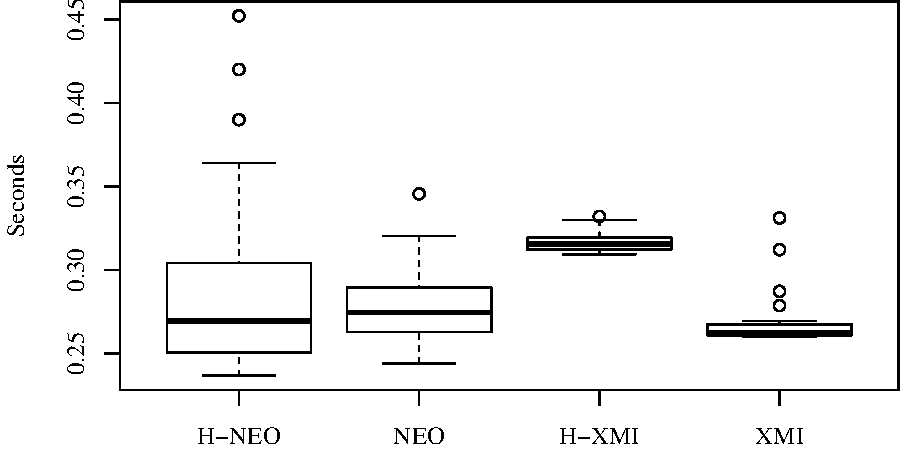
\includegraphics[width=\linewidth]{images/load_time_epsilon}
    \caption{Hybrid vs. state-based model persistence on model loading time for the Epsilon project.}
            \label{fig:load_time_epsilon}
\end{figure}

\begin{figure}[ht]
        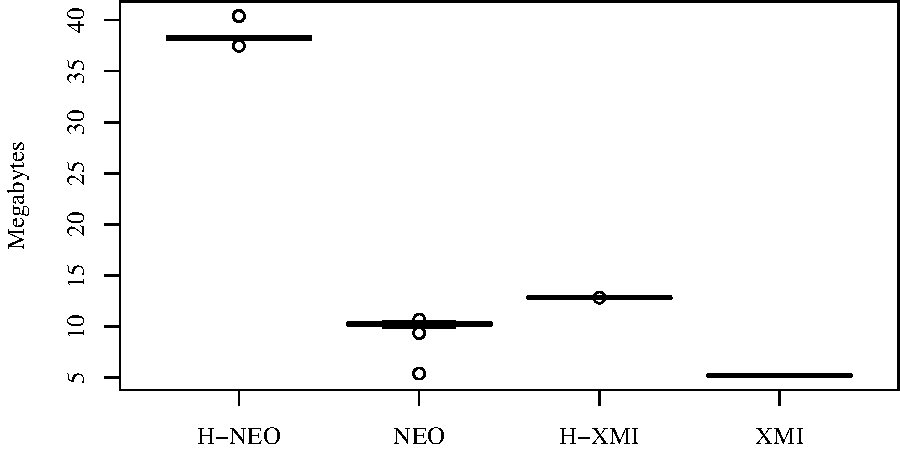
\includegraphics[width=\linewidth]{images/load_memory_epsilon}
        \caption{loading memory footprint}
    \caption{Hybrid vs. state-based model persistence on the memory footprint of loading a model for the Epsilon project.}
\label{fig:load_memory_epsilon}
\end{figure}

The model used for testing is the UML2 model of the Epsilon project that consists of 88,020 elements (the model is derived from the committed version number 940 from its Git repository). The results shows that the average loading time of Hybrid NeoEMF ($mean$ = 0.292, $sd$ = 0.061 seconds) is slightly slower than NeoEMF ($mean$ = 0.279, $sd$ = 0.023 seconds) but insignificant ($t$ = -0.97, $df$ = 26.94, $p$-value = 0.34). The slowdown is more significant ($t$ = -29.37, $df$ = 27.38, $p$-value $<$ 0.05) on Hybrid XMI ($mean$ = 0.873, $sd$ = 0.038 seconds) vs. XMI ($mean$ = 0.616, $sd$ = 0.015 seconds) but still in the order of less than 0.3 seconds.  

For the memory footprint after loading the model, Hybrid NeoEMF ($mean$ = 39, $sd$ = 0.9 MBs) uses more memory than NeoEMF ($mean$ = 10, $sd$ = 1.1 MBs) significantly ($t$ = -94.6, $df$ = 38.4, $p$-value $<$ 0.05). The similar significant increase on memory footprint ($t$ = -38131, $df$ = 25.8, $p$-value $<$ 0.05) also applies to Hybrid XMI ($mean$ = 12.8, $sd$ = 0.0 MBs) vs. XMI ($mean$ = 5.2, $sd$ = 0.0 MBs) when loading the model.  

\begin{figure}[ht]
    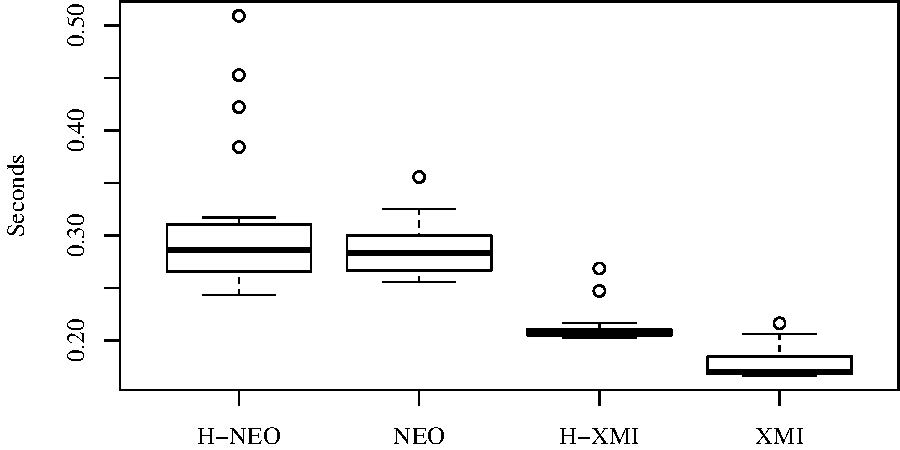
\includegraphics[width=\linewidth]{images/load_time_bpmn2}
    \caption{Hybrid vs. state-based model persistence on model loading time for the BPMN2 project.}
    \label{fig:load_time_bpmn2}
\end{figure}

\begin{figure}[ht]
    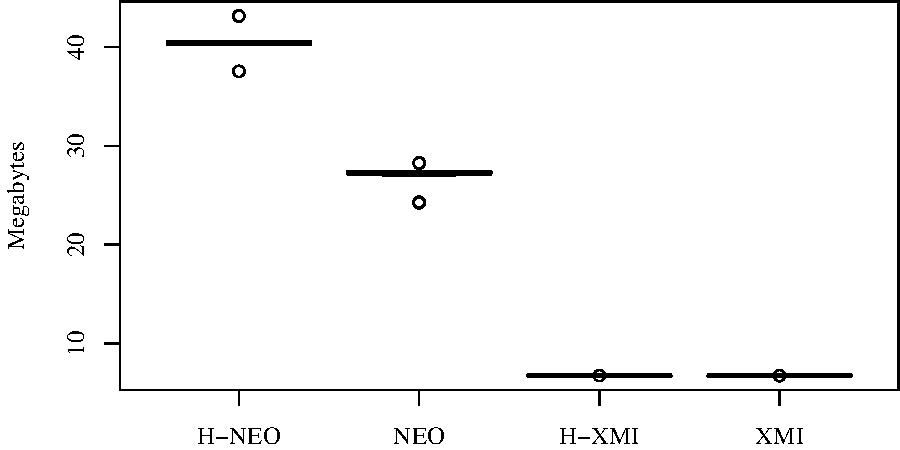
\includegraphics[width=\linewidth]{images/load_memory_bpmn2}
    \caption{loading memory footprint}
    \caption{Hybrid vs. state-based model persistence on the memory footprint of loading a model for the BPMN2 project.}
    \label{fig:load_memory_bpmn2}
\end{figure}


\subsubsection{BPMN2 Project}
\label{sec:model_loading_time_bpmn2}
We also perform the same evaluation on the UML2 model of the BPMN2 project that consists of 62,062 elements (the model is derived from the committed version number 192 from its Git repository). For this model, the results shows that the average loading time of Hybrid NeoEMF ($mean$ = 0.308, $sd$ = 0.071 seconds) is slightly slower than NeoEMF ($mean$ = 0.286, $sd$ = 0.025 seconds) but insignificant ($t$ = -1.39, $df$ = 26.10, $p$-value = 0.18). The slowdown is more significant ($t$ = -6.85, $df$ = 41.97, $p$-value $<$ 0.05) on Hybrid XMI ($mean$ = 0.212, $sd$ = 0.016 seconds) vs. XMI ($mean$ = 0.179, $sd$ = 0.016 seconds) but still in the order of less than 0.04 seconds.  

For the memory footprint after loading the model, Hybrid NeoEMF ($mean$ = 40.78, $sd$ = 1.29 MBs) uses more memory than NeoEMF ($mean$ = 27.20, $sd$ = 1.05 MBs) significantly ($t$ = -38.3, $df$ = 40.25, $p$-value $<$ 0.05). However, the increase of memory footprint is insignificant ($t$ = -0.42, $df$ = 27.79, $p$-value $<$ 0.68) for Hybrid XMI ($mean$ = 6.73374, $sd$ = 1.29305 MBs) vs. XMI ($mean$ = 6.73367, $sd$ = 0.00056 MBs) when loading the model.  

\subsubsection{Wikipedia Article}
\label{sec:model_loading_time_wikipedia}

\begin{figure}[ht]
    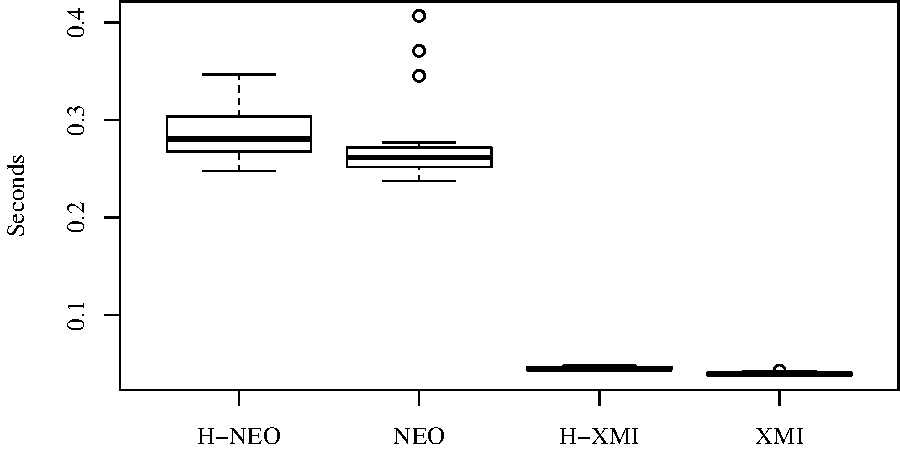
\includegraphics[width=\linewidth]{images/load_time_wikipedia}
    \caption{Hybrid vs. state-based model persistence on model loading time for the Wikipedia article.}
    \label{fig:load_time_wikipedia}
\end{figure}

\begin{figure}[ht]
    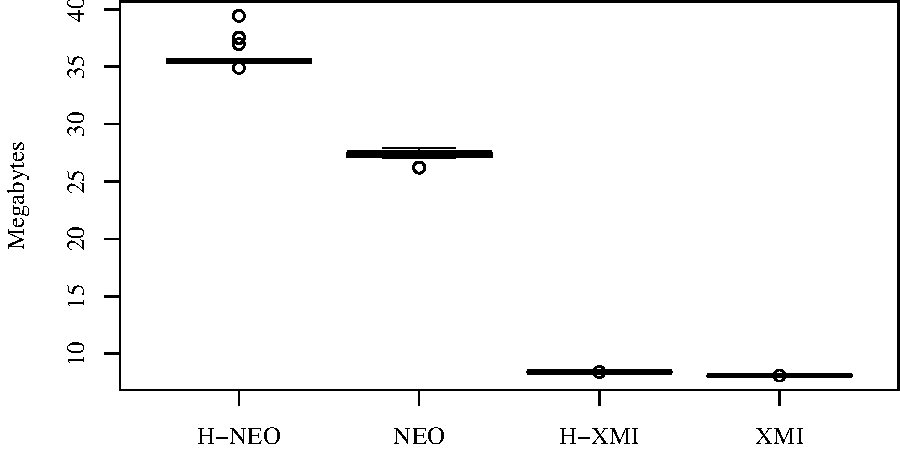
\includegraphics[width=\linewidth]{images/load_memory_wikipedia}
    \caption{loading memory footprint}
    \caption{Hybrid vs. state-based model persistence on the memory footprint of loading a model for the Wikipedia article.}
    \label{fig:load_memory_wikipedia}
\end{figure}

We also perform the evaluation on the ModiscoXML model of the Wikipedia's United States article project that consists of 13,122 elements (the model is derived from the version number 10,187 of its online page). For this model, the results shows that the average loading time of Hybrid NeoEMF ($mean$ = 0.287, $sd$ = 0.028 seconds) is slightly slower than NeoEMF ($mean$ = 0.275, $sd$ = 0.001 seconds) but insignificant ($t$ = -1.11, $df$ = 35.84, $p$-value = 0.28). The slowdown is more significant ($t$ = -13.83, $df$ = 41.98, $p$-value $<$ 0.05) on Hybrid XMI ($mean$ = 0.045, $sd$ = 0.001 seconds) vs. XMI ($mean$ = 0.040, $sd$ = 0.001 seconds) but still in the order of less than 0.01 seconds.  

For the memory footprint after loading the model, Hybrid NeoEMF ($mean$ = 35.91, $sd$ = 1.03 MBs) uses more memory than NeoEMF ($mean$ = 27.25, $sd$ = 0.54 MBs) significantly ($t$ = -34.83, $df$ = 31.56, $p$-value $<$ 0.05). A significant increase on memory footprint ($t$ = -1279.9, $df$ = 41.12, $p$-value $<$ 0.05) also happens on Hybrid XMI ($mean$ = 8.4079, $sd$ = 0.0008 MBs) vs. XMI ($mean$ = 8.0933, $sd$ = 0.0009 MBs) when loading the model.  

\subsection{Model Saving Time and Memory Footprint}
\label{sec:model_saving_time}
In this section, we present the results our evaluation on the time and memory footprint for the hybrid model persistence to save a change made to the model.

\subsubsection{Epsilon Project}
\label{sec:model_saving_time_epsilon}

\begin{figure}[ht]
    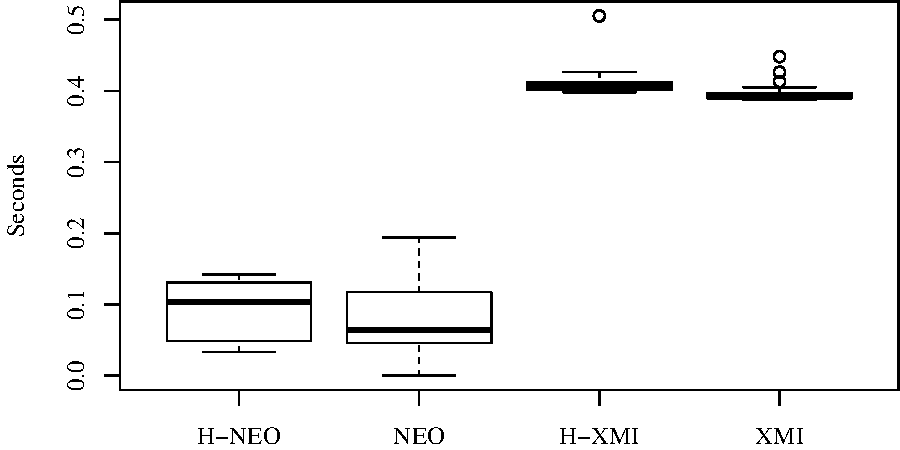
\includegraphics[width=\linewidth]{images/save_time_epsilon}
    \caption{Hybrid vs. state-based model persistence on model saving time.}
    \label{fig:save_time_epsilon}
\end{figure}

\begin{figure}[ht]
    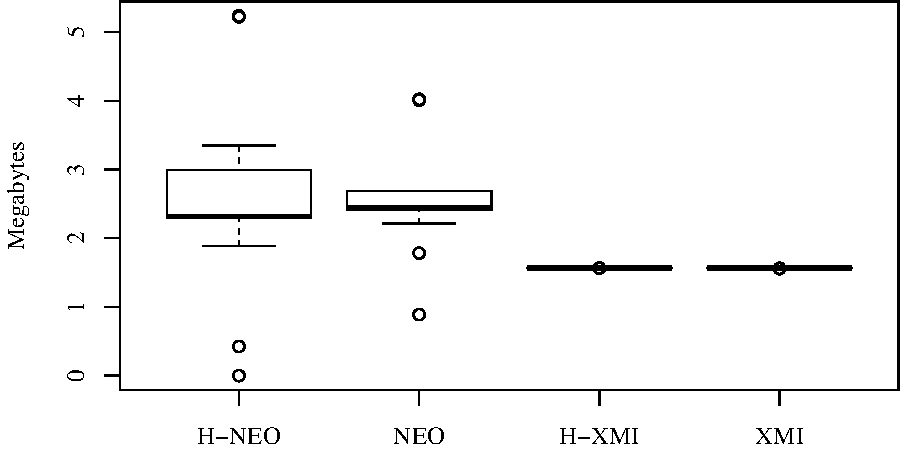
\includegraphics[width=\linewidth]{images/save_memory_epsilon}
    \caption{Hybrid vs. state-based model persistence on the memory footprint of saving a model.}
    \label{fig:save_memory_epsilon}
\end{figure}

Using the same UML2 model version 940 of the Epsilon project, the results shows that the average saving time for each change made to Hybrid NeoEMF ($mean$ = 0.0892, $sd$ = 0.0421 seconds) is slightly slower than the one made to NeoEMF ($mean$ = 0.0829, $sd$ = 0.0494 seconds) but insignificant ($t$ = -0.45, $df$ = 40.97, $p$-value = 0.65). The slowdown is more significant ($t$ = -2.5, $df$ = 36.1, $p$-value $<$ 0.05) on Hybrid XMI ($mean$ = 0.411, $sd$ = 0.023 seconds) vs. XMI ($mean$ = 0.397, $sd$ = 0.015 seconds) but still in the order of less than 0.02 seconds.  

For the memory footprint after saving a change made to the model, Hybrid NeoEMF ($mean$ = 2.64, $sd$ = 1.29 MBs) uses more memory than NeoEMF ($mean$ = 2.61, $sd$ = 0.78 MBs) but still at the insignificant level ($t$ = -0.14, $df$ = 34.67, $p$-value $=$ 0.89). Hybrid XMI ($mean$ = 1.56355, $sd$ = 0.0005 MBs) also uses more memory than XMI ($mean$ = 1.56326, $sd$ = 0.0018 MBs) when loading the model but also still at the insignificant level ($t$ = -0.76, $df$ = 23.8, $p$-value $=$ 0.46).  

\subsubsection{BPMN2 Project}
\label{sec:model_saving_time_bpmn2}

\begin{figure}[ht]
    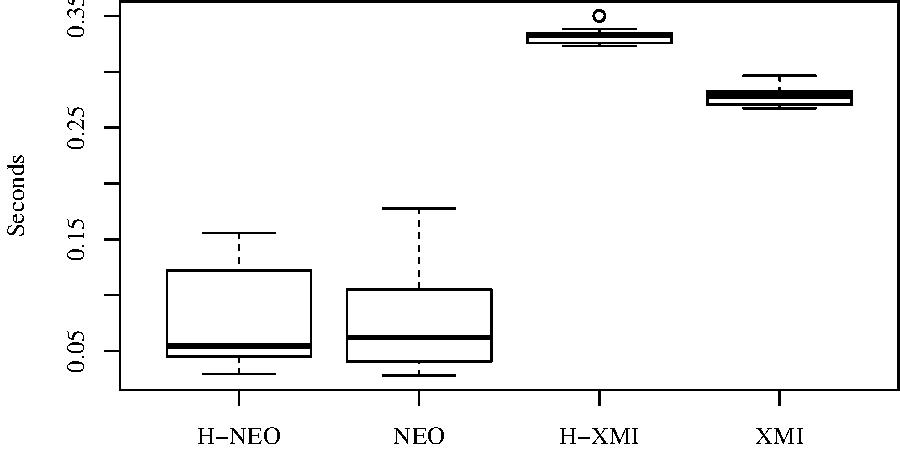
\includegraphics[width=\linewidth]{images/save_time_bpmn2}
    \caption{Hybrid vs. state-based model persistence on model saving time for the BPMN2 project.}
    \label{fig:save_time_bpmn2}
\end{figure}

\begin{figure}[ht]
    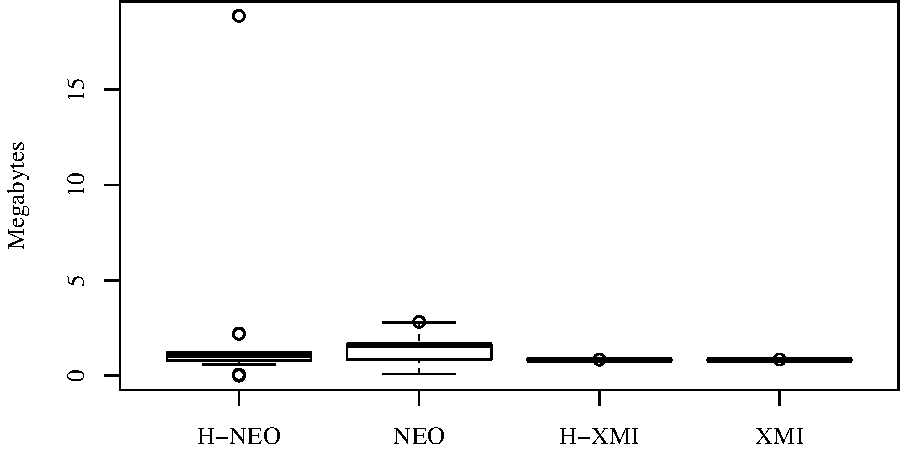
\includegraphics[width=\linewidth]{images/save_memory_bpmn2}
    \caption{Hybrid vs. state-based model persistence on the memory footprint of saving a model for the BPMN2 project.}
    \label{fig:save_memory_bpmn2}
\end{figure}

Using the same UML2 model version 192 of the BPMN2 project, the results shows that the average saving time for each change made to Hybrid NeoEMF ($mean$ = 0.0777, $sd$ = 0.0424 seconds) is slightly slower than the one made to NeoEMF ($mean$ = 0.0775, $sd$ = 0.0452 seconds) but insignificant ($t$ = -0.02, $df$ = 41.83, $p$-value = 0.99). The slowdown is more significant ($t$ = -23.85, $df$ = 39.93, $p$-value $<$ 0.05) on Hybrid XMI ($mean$ = 0.33, $sd$ = 0.007 seconds) vs. XMI ($mean$ = 0.28, $sd$ = 0.008 seconds) but still in the order of less than 0.06 seconds.  

For the memory footprint after saving a change made to the model, Hybrid NeoEMF ($mean$ = 1.86, $sd$ = 3.86 MBs) uses more memory than NeoEMF ($mean$ = 1.52, $sd$ = 0.77 MBs) but still at the insignificant level ($t$ = -0.4, $df$ = 22.66, $p$-value $=$ 0.69). Hybrid XMI ($mean$ = 0.8378, $sd$ = 0.00361 MBs) also uses more memory than XMI ($mean$ = 0.8375, $sd$ = 0.00362 MBs) when loading the model but also still at the insignificant level ($t$ = -0.22, $df$ = 42, $p$-value $=$ 0.83).  

\subsubsection{Wikipedia Article}
\label{sec:model_saving_time_wikipedia}

\begin{figure}[ht]
    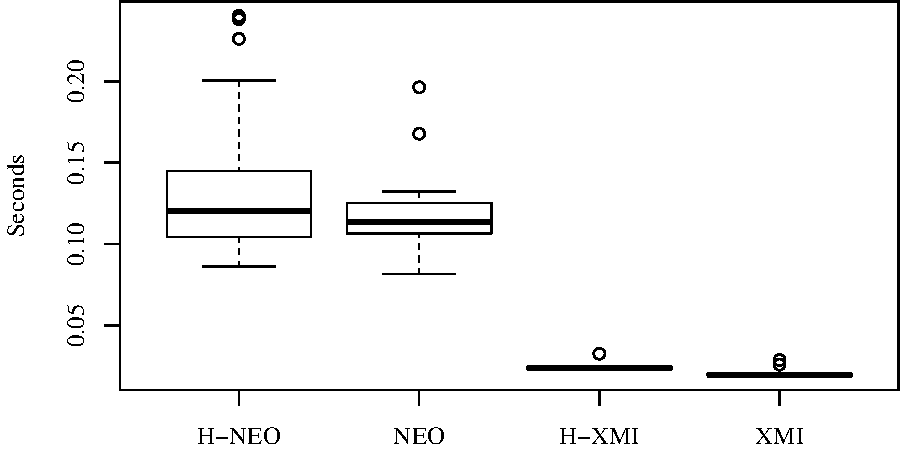
\includegraphics[width=\linewidth]{images/save_time_wikipedia}
    \caption{Hybrid vs. state-based model persistence on model saving time for the Wikipedia article.}
    \label{fig:save_time_wikipedia}
\end{figure}

\begin{figure}[ht]
    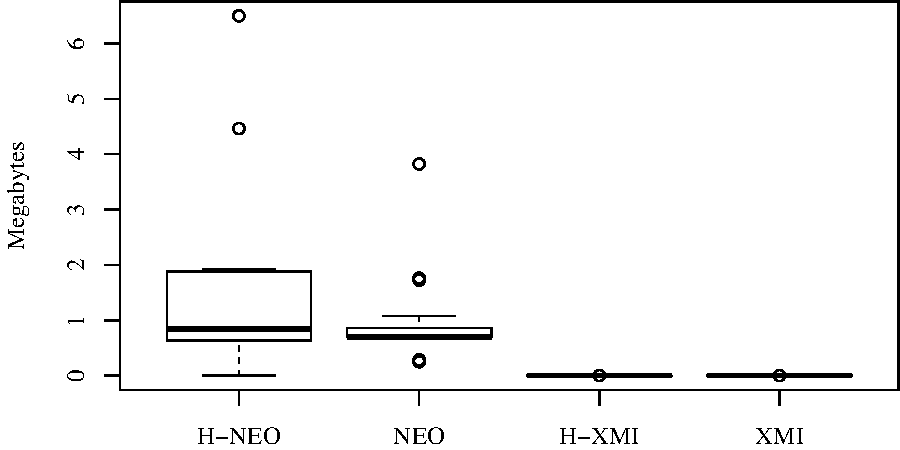
\includegraphics[width=\linewidth]{images/save_memory_wikipedia}
    \caption{Hybrid vs. state-based model persistence on the memory footprint of saving a model for the Wikipedia article.}
    \label{fig:save_memory_wikipedia}
\end{figure}

Using the same MoDiscoXML model version 10,187 of the Wikipedia's United States article, the results shows that the average saving time for each change made to Hybrid NeoEMF ($mean$ = 0.135, $sd$ = 0.048 seconds) is slightly slower than the one made to NeoEMF ($mean$ = 0.120, $sd$ = 0.024 seconds) but insignificant ($t$ = -1.33, $df$ = 30.71, $p$-value = 0.19). The slowdown is more significant ($t$ = -5.9, $df$ = 40.69, $p$-value $<$ 0.05) on Hybrid XMI ($mean$ = 0.024, $sd$ = 0.048 seconds) vs. XMI ($mean$ = 0.020, $sd$ = 0.002 seconds) but still in the order of less than 0.006 seconds.

For the memory footprint after saving a change made to the model, Hybrid NeoEMF ($mean$ = 1.32, $sd$ = 1.51 MBs) uses more memory than NeoEMF ($mean$ = 0.97, $sd$ = 0.76 MBs) but still at the insignificant level ($t$ = -0.97, $df$ = 30.9, $p$-value $=$ 0.34). Hybrid XMI ($mean$ = 0.0010, $sd$ = 0.00044 MBs) also uses more memory than XMI ($mean$ = 0.0005, $sd$ = 0.00001 MBs) when loading the model and at the significant level ($t$ = -5.0, $df$ = 21.08, $p$-value $<$ 0.05).  

\subsection{Storage Space Usage}
\label{sec:storage_space_usage}
We also performed evaluation on storage space usage of the hybrid model persistence. In addition to the CBP generated from the Epsilon project, we also generated two CBPs from the BPMN2 project \cite{eclipse2017bpmn2,eclipse2018bpmn2git}, and the United States (US) article \cite{wikipedia2018us} on Wikipedia (the article is further referred as Wikipedia). We generated the committed versions of the BPMN2 project as UML2 models \cite{eclipse2017uml2} and the versions of the Wikipedia article as MoDiscoXML models \cite{eclipse2018modiscoxml}.

\begin{table} [ht]
    \centering
    \caption{Space Usage for the Epsilon project. The CBP were generated from  version 1 to 940 of the project.}
    \label{table:space_usage_epsilon}
    \begin{tabular}{ p{0.1\linewidth} p{0.1\linewidth} p{0.12\linewidth} p{0.13\linewidth} p{0.26\linewidth} }
    \hline 
    \textbf{Type} & \textbf{Element Count} & \textbf{Event Count} & \textbf{Space Size} & \textbf{Average Space Size} \\
    \hline 
    XMI & 88,020 &  & 9.44 MBs & 112 bytes / element  \\
    NeoEMF & 88,020 &  & 188 MBs & 2 KBs / element \\
    CBP &  & 4,307,051 & 406 MBs &  98 bytes / event \\
    \hline 
    \end{tabular}
\end{table}

\begin{table} [ht]
    \centering
    \caption{Space Usage for the BPMN2 project. The CBP were generated from version 1 to 192 of the project.}
    \label{table:space_usage_bpmn2}
    \begin{tabular}{ p{0.1\linewidth} p{0.1\linewidth} p{0.12\linewidth} p{0.13\linewidth} p{0.26\linewidth} }
        \hline 
        \textbf{Type} & \textbf{Element Count} & \textbf{Event Count} & \textbf{Space Size} & \textbf{Average Space Size} \\
        \hline 
        XMI & 62,062 &  & 6.55 MBs & 110 bytes / element  \\
        NeoEMF & 62,062 &  & 134 MBs & 2 KBs / element \\
        CBP &  & 1,238,751 & 109 MBs &  92 bytes / event \\
        \hline 
    \end{tabular}
\end{table}

\begin{table} [ht]
    \centering
    \caption{Space Usage for the Wikipedia's US article. The CBP were generated from version 1 to 10,187 of the article.}
    \label{table:space_usage_wikipedia}
    \begin{tabular}{ p{0.1\linewidth} p{0.1\linewidth} p{0.12\linewidth} p{0.13\linewidth} p{0.26\linewidth} }
        \hline 
        \textbf{Type} & \textbf{Element Count} & \textbf{Event Count} & \textbf{Space Size} & \textbf{Average Space Size} \\
        \hline 
        XMI & 13,112 &  & 1.28 MBs & 102 bytes / element  \\
        NeoEMF & 13,112 &  & 31.8 MBs & 2 KBs / element \\
        CBP &  & 62,271,003 & 5.85 GBs &  98 bytes / event \\
        \hline 
    \end{tabular}
\end{table}

For the Epsilon project, we have successfully generated its CBP from version 1 up to number 940 of all its versions. For the BPMN2 project and Wikipedia article, we have successfully generated their CBPs up to version number 192 and 10,187 respectively. The details (element count, event count, space size, and average space size per element or event) of their models if persisted in XMI, NeoEMF, and CBP can be seen in Table \ref{table:space_usage_epsilon}, \ref{table:space_usage_bpmn2}, and \ref{table:space_usage_wikipedia}. Using the tables, we can estimate roughly the growth of the models that every additional element consumes more than around 102 bytes for XMI and 2KBs for NeoEMF. Every change made to the models consumes more than around 92 bytes per persisted event. With such rates, we can estimate roughly the space usage growth of the hybrid model persistence, and it is the combination of the change and state-based persistence.

\subsection{Change Detection}
\label{sec:change_detection}
In this section, we present the the evaluation of change-based persistence, as a component of the hybrid model persistence, on faster model change detection. In this evaluation, we used four versions of the the Epsilon project's UML2 model: committed version 8, 44, 181, and 388. Table \ref{table:version_description} shows their description.

\begin{table}[ht]
    \centering
    \caption{Description of version 8, 44, 181, and 388 of the Epsilon project's UML2 model.}
    \label{table:version_description}
    \begin{tabular}{ r r r r r}
        \hline 
        \textbf{\thead{Versions}} & \textbf{\thead{Element\\Counts}} & \textbf{\thead{Delta Elements\\(from ver. 8)}} & \textbf{\thead{Event\\Counts}} & \textbf{\thead{Delta Events\\(from ver. 8)}}  \\
        \hline 
        8	& 25,993 & 0	& 90,888 & 0\\
        44	& 31,240 & 5,247	& 166,659 & 75,771\\
        181	& 34,196 & 8,203	& 250,073 & 159,185\\
        388	& 48,482 & 22,489 & 332,315 & 241,427\\
        \hline 
    \end{tabular}
\end{table}

As the scenario for the evaluation, we wanted to identify which elements in the older model (the left-side model) that did not exist any more in the newer model (right-side model). Thus, we paired up model version 8 to 44, 8 to 181, and 8 to 383, and used them as dataset. We used two methods to identify the deleted elements. First, we iterated through events in the change-based persistence of the pairs' hybrid-model persistence to identify them (\emph{the hybrid method}). Second, we performed model-to-model comparison between the two states of the paired versions using EMF Compare to identify the deleted elements (\emph{the state-based method}). We compared both methods on the the time they required to identify all the deleted elements. We performed measurement 22 times for each pair and method to calculate the time. Fig. \ref{fig:delete_detection_epsilon_average} shows the result of the comparison. 

\begin{figure}[ht]
    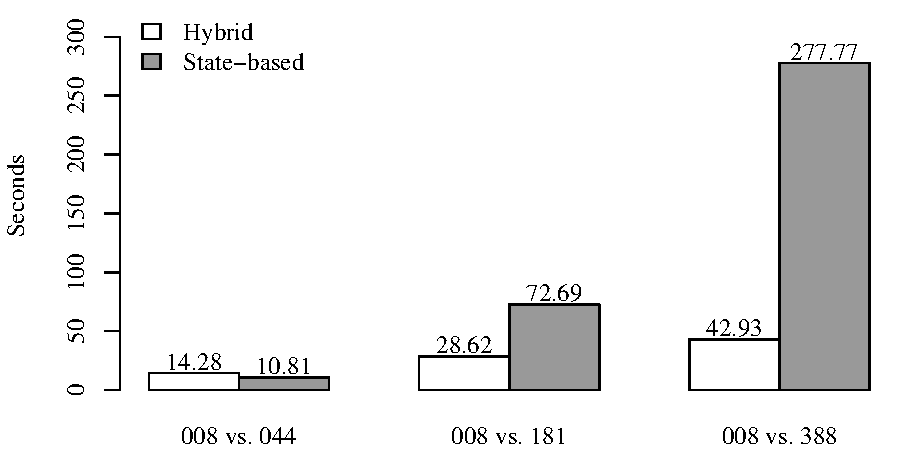
\includegraphics[width=\linewidth]{images/delete_detection_epsilon_average}
    \caption{The time required for hybrid and state-based methods on detecting older version's elements that do not exist in newer versions.}
    \label{fig:delete_detection_epsilon_average}
\end{figure}

On the 008 vs. 044 pair, the state-based method ($mean$ = 10.81 , $sd$ = 0.16 seconds) completes the change detection 3.47 seconds faster than the hybrid method ($mean$ = 14.28, $sd$ = 0.36 seconds), while on the 008 vs. 181 pair, the hybrid method ($mean$ = 28.62 , $sd$ = 0.17 seconds)  performs better, 44.07 seconds faster, than the state-based method ($mean$ = 72.69, $sd$ = 1.28 seconds). The hybrid method considerably outperforms the state-based method on the 008 vs. 388 pair. The hybrid method ($mean$ = 42.93, $sd$ = 0.18 seconds) is 234.84 seconds faster than the change-based method ($mean$ = 277.77, $sd$ = 4.70 seconds). Considering the increasing number of elements and events in Table \ref{table:version_description}, the change identification time of the hybrid method tends to grow linearly as the number of events increases, which is an advantage for faster change detection, compared to the stated-based method that tends to grow exponentially as the number of elements increases.

\subsection{Threats to Validity and Limitations}
\label{sec:threats_to_validity_and_limitations}
In this work, we have only tested the hybrid model persistence approach on synthesised models which may not be representative of the characteristics of models made by a person or people in the real-world. The evaluation also has not been tested on big models -- models that contain more than a million elements and events. Moreover, our model comparison evaluation is limited only to detecting changes for versions of model that are developed sequentially, not in paralel. Versions of a model developed in parallel might have conflicts between them which requires conflict resolution before merging.

\section{Discussion}
\label{sec:discussion}
The evaluation result on change detection in Section \ref{sec:change_detection} shows that model change detection in hybrid model persistence can be performed faster than using naive model comparison approach in state-based persistence. This is possible because elements and features that have been modified can be directly identified through the events recorded in its change-based persistence without necessity to compare the models element-by-element. The use of state-based persistence in hybrid model persistence enables faster loading of model, as shown by the result of loading time evaluation in Section \ref{sec:model_loading_time}, without having to replay all the changes persisted in its change-based persistence -- the main challenge change-based approach \cite{mens2002state}. 
The hybrid model persistence only performs slightly slower and insignificant on model loading compared to loading a model in state-based persistence. The slight slowndown also appears on model saving, but also at the insignificant level as reported in Section \ref{sec:model_saving_time}, because changes have to be persisted into two representation, state-based and change-based. 

The subtle drawbacks of hybrid model persistence is that it consumes more memory when loading and saving and storage space for persisting models compared to state-based representation only (see Section \ref{sec:model_loading_time}, \ref{sec:model_saving_time}, and \ref{sec:storage_space_usage}). However, considering the cost of main memory and storage, this trade-off will be paid off.

\section{Related Work}
\label{sec:related_work}
Change-based persistence-like approach has been used widely in many incremental projects (e.g IncQuery \cite{DBLP:conf/ecmdafa/RathHV12}, ReactiveATL \cite{DBLP:conf/ecmdafa/OgunyomiRK15}) usually by harnessing the notification facilities that already provided by the platform (e.g. Eclipse). It is also has been applied in other artefacts, such as software \cite{DBLP:journals/entcs/RobbesL07}, database \cite{DBLP:conf/sde/LippeO92}, hierarchical documents \cite{DBLP:conf/caise/IgnatN05}, model repository and version control \cite{koegel2010emfstore}. The approach is faster for detecting changes \cite{DBLP:conf/edoc/KoegelHLHD10}, more accurate and carries semantic information \cite{DBLP:journals/entcs/RobbesL07,DBLP:conf/sde/LippeO92,DBLP:conf/caise/IgnatN05,mens2002state}, faster and more accurate for comparison and merging \cite{DBLP:conf/sde/LippeO92,DBLP:conf/caise/IgnatN05,koegel2010emfstore}, and information carried is useful for analytics \cite{DBLP:journals/entcs/RobbesL07}.

There are several alternative approaches to the standard XMI format for persisting models in state-based. Such approaches harness relational and NoSQL databases as backends. EMF Teneo \cite{eclipse2017teneo} persists models into relational databases, while NeoEMF \cite{daniel2016neoemf} and Morsa \cite{DBLP:conf/models/Espinazo-PaganCM11}, use graph and document databases as their backends. However, these approaches do not have built-in support for model versioning, and storing models in the form of folders/binary files is poorly fit with text-based version control systems, such as SVN and Git. Besides supporting databases as model persistence's backends, Connected Data Objects (CDO) \cite{eclipse2017cdo} also provides collaboration facilities. However, it requires separation of version control systems (e.g. a CDO repository for models and a Git repository for code) in software development process, which causes administration and fragmentation challenges  \cite{barmpis2014evaluation}. Other model-specific version control systems, such as EMFStore \cite{koegel2010emfstore}, also faces similar challenges.

\section{Conclusions and Future Work}
\label{sec:conlcusions_and_future_work}
In this paper, we propose a hybrid model persistence and evaluate its impact on time and memory footprint for model loading and saving, storage space usage, and detecting changes of versions of the same model. Based on the evaluation results, the hybrid model persistence provides considerable benefits on model loading time and change detection with acceptable trade-off on memory footprint and storage space usage.

For our future work, we plan to evaluate the hybrid model persistence on big models, and perform simulations where software modellers are asked to construct several models. The changes of the models will be recorded into change-based model representations and upscaled to better reflect changes of models in the real-world. We also plan to develop a solution to compare and merge different versions of a change-based model that are developed in parallel.  

% An example of a floating figure using the graphicx package.
% Note that \label must occur AFTER (or within) \caption.
% For figures, \caption should occur after the \includegraphics.
% Note that IEEEtran v1.7 and later has special internal code that
% is designed to preserve the operation of \label within \caption
% even when the captionsoff option is in effect. However, because
% of issues like this, it may be the safest practice to put all your
% \label just after \caption rather than within \caption{}.
%
% Reminder: the "draftcls" or "draftclsnofoot", not "draft", class
% option should be used if it is desired that the figures are to be
% displayed while in draft mode.
%
%\begin{figure}[!t]
%\centering
%\includegraphics[width=2.5in]{myfigure}
% where an .eps filename suffix will be assumed under latex, 
% and a .pdf suffix will be assumed for pdflatex; or what has been declared
% via \DeclareGraphicsExtensions.
%\caption{Simulation results for the network.}
%\label{fig_sim}
%\end{figure}

% Note that the IEEE typically puts floats only at the top, even when this
% results in a large percentage of a column being occupied by floats.


% An example of a double column floating figure using two subfigures.
% (The subfig.sty package must be loaded for this to work.)
% The subfigure \label commands are set within each subfloat command,
% and the \label for the overall figure must come after \caption.
% \hfil is used as a separator to get equal spacing.
% Watch out that the combined width of all the subfigures on a 
% line do not exceed the text width or a line break will occur.
%
%\begin{figure\\}[!t]
%\centering
%\subfloat[Case I]{\includegraphics[width=2.5in]{box}%
%\label{fig_first_case}}
%\hfil
%\subfloat[Case II]{\includegraphics[width=2.5in]{box}%
%\label{fig_second_case}}
%\caption{Simulation results for the network.}
%\label{fig_sim}
%\end{figure\\}
%
% Note that often IEEE papers with subfigures do not employ subfigure
% captions (using the optional argument to \subfloat[]), but instead will
% reference/describe all of them (a), (b), etc., within the main caption.
% Be aware that for subfig.sty to generate the (a), (b), etc., subfigure
% labels, the optional argument to \subfloat must be present. If a
% subcaption is not desired, just leave its contents blank,
% e.g., \subfloat[].


% An example of a floating table. Note that, for IEEE style tables, the
% \caption command should come BEFORE the table and, given that table
% captions serve much like titles, are usually capitalized except for words
% such as a, an, and, as, at, but, by, for, in, nor, of, on, or, the, to
% and up, which are usually not capitalized unless they are the first or
% last word of the caption. Table text will default to \footnotesize as
% the IEEE normally uses this smaller font for tables.
% The \label must come after \caption as always.
%
%\begin{table}[!t]
%% increase table row spacing, adjust to taste
%\renewcommand{\arraystretch}{1.3}
% if using array.sty, it might be a good idea to tweak the value of
% \extrarowheight as needed to properly center the text within the cells
%\caption{An Example of a Table}
%\label{table_example}
%\centering
%% Some packages, such as MDW tools, offer better commands for making tables
%% than the plain LaTeX2e tabular which is used here.
%\begin{tabular}{|c||c|}
%\hline
%One & Two\\
%\hline
%Three & Four\\
%\hline
%\end{tabular}
%\end{table}


% Note that the IEEE does not put floats in the very first column
% - or typically anywhere on the first page for that matter. Also,
% in-text middle ("here") positioning is typically not used, but it
% is allowed and encouraged for Computer Society conferences (but
% not Computer Society journals). Most IEEE journals/conferences use
% top floats exclusively. 
% Note that, LaTeX2e, unlike IEEE journals/conferences, places
% footnotes above bottom floats. This can be corrected via the
% \fnbelowfloat command of the stfloats package.



% conference papers do not normally have an appendix


% use section\\ for acknowledgment
\section*{Acknowledgment}
This research is part of a doctoral programme funded by \emph{Lembaga Pengelola Dana Pendidikan Indonesia} (Indonesia Endowment Fund for Education).

% trigger a \newpage just before the given reference
% number - used to balance the columns on the last page
% adjust value as needed - may need to be readjusted if
% the document is modified later
%\IEEEtriggeratref{30}
% The "triggered" command can be changed if desired:
%\IEEEtriggercmd{\enlargethispage{-5in}}

% references section

% can use a bibliography generated by BibTeX as a .bbl file
% BibTeX documentation can be easily obtained at:
% http://mirror.ctan.org/biblio/bibtex/contrib/doc/
% The IEEEtran BibTeX style support page is at:
% http://www.michaelshell.org/tex/ieeetran/bibtex/
%\bibliographystyle{IEEEtran}
% argument is your BibTeX string definitions and bibliography database(s)
%\bibliography{IEEEabrv,../bib/paper}
%
% <OR> manually copy in the resultant .bbl file
% set second argument of \begin to the number of references
% (used to reserve space for the reference number labels box)
%\begin{thebibliography}{1}
%
%\bibitem{IEEEhowto:kopka}
%H.~Kopka and P.~W. Daly, \emph{A Guide to \LaTeX}, 3rd~ed.\hskip 1em plus
%  0.5em minus 0.4em\relax Harlow, England: Addison-Wesley, 1999.
%
%\end{thebibliography}

\bibliographystyle{IEEEtran}
\bibliography{references}



% that's all folks
\end{document}